\documentclass[man,floatsintext]{apa6}
\usepackage{lmodern}
\usepackage{amssymb,amsmath}
\usepackage{ifxetex,ifluatex}
\usepackage{fixltx2e} % provides \textsubscript
\ifnum 0\ifxetex 1\fi\ifluatex 1\fi=0 % if pdftex
  \usepackage[T1]{fontenc}
  \usepackage[utf8]{inputenc}
\else % if luatex or xelatex
  \ifxetex
    \usepackage{mathspec}
  \else
    \usepackage{fontspec}
  \fi
  \defaultfontfeatures{Ligatures=TeX,Scale=MatchLowercase}
\fi
% use upquote if available, for straight quotes in verbatim environments
\IfFileExists{upquote.sty}{\usepackage{upquote}}{}
% use microtype if available
\IfFileExists{microtype.sty}{%
\usepackage{microtype}
\UseMicrotypeSet[protrusion]{basicmath} % disable protrusion for tt fonts
}{}
\usepackage{hyperref}
\hypersetup{unicode=true,
            pdftitle={A pre-registered multi-site study investigating the effects of inhibitory control training on automatic action tendencies for unhealthy foods},
            pdfauthor={Loukia Tzavella, Ernst-August Doelle, Christopher D. Chambers, Natalia Lawrence, Katherine S. Button, Elizabeth Hart, Natalie Holmes, Kimberley Houghton, Nina Badkar, Ellie Macey, Amy-Jayne Braggins, Felicity Murray, \& Rachel C. Adams},
            pdfkeywords={inhibitory control training, go/no-go, foods, devaluation, action tendencies, approach bias},
            pdfborder={0 0 0},
            breaklinks=true}
\urlstyle{same}  % don't use monospace font for urls
\usepackage{graphicx,grffile}
\makeatletter
\def\maxwidth{\ifdim\Gin@nat@width>\linewidth\linewidth\else\Gin@nat@width\fi}
\def\maxheight{\ifdim\Gin@nat@height>\textheight\textheight\else\Gin@nat@height\fi}
\makeatother
% Scale images if necessary, so that they will not overflow the page
% margins by default, and it is still possible to overwrite the defaults
% using explicit options in \includegraphics[width, height, ...]{}
\setkeys{Gin}{width=\maxwidth,height=\maxheight,keepaspectratio}
\IfFileExists{parskip.sty}{%
\usepackage{parskip}
}{% else
\setlength{\parindent}{0pt}
\setlength{\parskip}{6pt plus 2pt minus 1pt}
}
\setlength{\emergencystretch}{3em}  % prevent overfull lines
\providecommand{\tightlist}{%
  \setlength{\itemsep}{0pt}\setlength{\parskip}{0pt}}
\setcounter{secnumdepth}{0}
% Redefines (sub)paragraphs to behave more like sections
\ifx\paragraph\undefined\else
\let\oldparagraph\paragraph
\renewcommand{\paragraph}[1]{\oldparagraph{#1}\mbox{}}
\fi
\ifx\subparagraph\undefined\else
\let\oldsubparagraph\subparagraph
\renewcommand{\subparagraph}[1]{\oldsubparagraph{#1}\mbox{}}
\fi

%%% Use protect on footnotes to avoid problems with footnotes in titles
\let\rmarkdownfootnote\footnote%
\def\footnote{\protect\rmarkdownfootnote}


  \title{A pre-registered multi-site study investigating the effects of inhibitory control training on automatic action tendencies for unhealthy foods}
    \author{Loukia Tzavella\textsuperscript{1}, Ernst-August Doelle\textsuperscript{1,2}, Christopher D. Chambers\textsuperscript{1}, Natalia Lawrence\textsuperscript{2}, Katherine S. Button\textsuperscript{3}, Elizabeth Hart\textsuperscript{4}, Natalie Holmes\textsuperscript{4}, Kimberley Houghton\textsuperscript{4}, Nina Badkar\textsuperscript{2}, Ellie Macey\textsuperscript{2}, Amy-Jayne Braggins\textsuperscript{3}, Felicity Murray\textsuperscript{2}, \& Rachel C. Adams\textsuperscript{1}}
    \date{}
  
\shorttitle{ICT effects on food action tendencies}
\affiliation{
\vspace{0.5cm}
\textsuperscript{1} Cardiff University Brain Research Imaging Centre, CF24 4HQ, UK\\\textsuperscript{2} School of Psychology, University of Exeter, EX4 4QG, UK\\\textsuperscript{3} Department of Psychology, University of Bath, BS2 7AY, UK\\\textsuperscript{4} School of Psychology, Cardiff University, CF10 3AT, UK}
\keywords{inhibitory control training, go/no-go, foods, devaluation, action tendencies, approach bias\newline\indent Word count: X}
\usepackage{csquotes}
\usepackage{upgreek}
\captionsetup{font=singlespacing,justification=justified}

\usepackage{longtable}
\usepackage{lscape}
\usepackage{multirow}
\usepackage{tabularx}
\usepackage[flushleft]{threeparttable}
\usepackage{threeparttablex}

\newenvironment{lltable}{\begin{landscape}\begin{center}\begin{ThreePartTable}}{\end{ThreePartTable}\end{center}\end{landscape}}

\makeatletter
\newcommand\LastLTentrywidth{1em}
\newlength\longtablewidth
\setlength{\longtablewidth}{1in}
\newcommand{\getlongtablewidth}{\begingroup \ifcsname LT@\roman{LT@tables}\endcsname \global\longtablewidth=0pt \renewcommand{\LT@entry}[2]{\global\advance\longtablewidth by ##2\relax\gdef\LastLTentrywidth{##2}}\@nameuse{LT@\roman{LT@tables}} \fi \endgroup}


\usepackage{lineno}

\linenumbers
\usepackage{xcolor}
\usepackage{multicol}
\usepackage{enumitem}

\setlist{nosep}
\usepackage[font=footnotesize,labelfont=bf]{caption}
\usepackage{float}
\usepackage{amsmath}
\usepackage{soul}
\usepackage{caption}

\authornote{The research project was conducted as part of the GW4 Undergraduate Psychology Consortium 2017/2018. This project was partially supported by the European Research Council (Consolidator 647893; C.D.C.). We gratefully acknowledge Teaching Development Funding, from the faculty of Humanities and Social Sciences at the University of Bath for funding travel and room hire costs for the consortium meetings.

Correspondence concerning this article should be addressed to Loukia Tzavella, Cardiff University Brain Research Imaging Centre, CF24 4HQ, UK. E-mail: \href{mailto:tzavellal@cardiff.ac.uk}{\nolinkurl{tzavellal@cardiff.ac.uk}}}



\begin{document}
\maketitle

\#Introduction \{\#introduction\}

\par

There is an increasing interest in the development of behaviour change interventions for eating behaviours that may arise in an \enquote{obesogenic environment}, such as overeating. These interventions largely focus on the cognitive processes that are responsible for enhancing an individual's self-control, such as response inhibition. There has been considerable evidence to suggest that such interventions can result in reduced food consumption in the laboratory (see A. Jones et al., 2016a; Allom, Mullan, \& Hagger, 2016 for meta-analyses). A common inhibitory control training (ICT) intervention has been adapted from the go/no-go paradigm, where participants are trained to inhibit their responses towards highly appetitive foods, and has been shown to reduce food intake (e.g., Houben \& Jansen, 2015; N. S. Lawrence et al., 2015a). A potential mechanism of action behind ICT effects on food consumption is stimulus devaluation, whereby the evaluations of appetitive foods are reduced during training to facilitate performance when response inhibition is required (e.g., Chen et al., 2016a). A possible explanation for this devaluation effect is provided by the Behaviour Stimulus Interaction (BSI) theory which posits that food stimuli are devalued when negative affect is induced to reduce the ongoing conflict between triggered approach reactions to appetitive foods and the need to inhibit responses towards those stimuli (Chen et al., 2016b; Veling, Holland, \& van Knippenberg, 2008; Veling et al., 2017). If the automatic action tendency to approach the food cue is reduced, the inhibition of responses in the ICT tasks can be facilitated. In this study we aimed to explore the interaction between inhibition and approach motivation further in relation to ICT outcomes. Although the BSI theory focuses on approach tendencies and not avoidance, we aimed to investigate both automatic action tendencies as an outcome of go/no-go training in addition to stimulus devaluation. Specifically, we tested whether go/no-go training changes approach and/or avoidance tendecies towards unhealthy foods associated with response inhibition.

\par

In dual-process model frameworks, behaviour is determined by the interaction of \texttt{impulsive\textquotesingle{},\ or\ automatic\ and}reflective', or controlled cognitive processes (Kakoschke, Kemps, \& Tiggemann, 2015; Strack \& Deutsch, 2004). The reflective system refers to our conscious and deliberate thoughts that result in reasoned actions which are in line with our long-term goals. The impulsive system, however, involves actions that occur without weighting any potential consequences and are driven by hedonic needs and desires. Eating behaviours that may give rise to obesity rates, such as overeating, may be explained by a weak reflective system and/or a strong impulsive system (e.g., Lawrence, Hinton, Parkinson, \& Lawrence, 2012; Nederkoorn, Coelho, Guerrieri, Houben, \& Jansen, 2012). \hl{I had a perfect reference for this - it's somewhere in my old notes and posters- find it!! and double-check references- also Rachel here had this:for a review see; Stice, Lawrence Kemps, \& Veling, 2016}. For instance, exposure to unhealthy appetitive food cues might trigger a conflict between automatic and controlled processing. Attentional (e.g., attending to the cue) and motivational (e.g., approaching appetitive food) processes would be automatic, while choosing an action towards these foods (e.g., eating vs not eating) while considering the compatibility of long-term goals (e.g., losing weight and eating unhealthy foods is not compatible) is a controlled process (Kakoschke et al., 2015). Indeed, it has been shown that overweight or obese individuals demonstrate poor self-control and increased impulsivity across a range of questionnaires and behavioural measures (e.g., Houben, Nederkoorn, \& Jansen, 2014; Lavagnino, Arnone, Cao, Soares, \& Selvaraj, 2016; Nederkoorn et al., 2012). Inhibitory control in relation to unhealthy eating patterns has generally been defined as \enquote{the ability to inhibit a behavioural impulse in order to attain higher-order goals, such as weight loss} (Houben, Nederkoorn, \& Jansen, 2012, p. 550). Strengthening the impulsive, or automatic, system may therefore involve enhancing response inhibition and reducing approach bias towards appetitive foods.

\par

In a typical ICT paradigm, participants are instructed to make a speeded choice response to healthy and unhealthy foods, but to withhold that response when a visual, or auditory, signal is presented. Signal-stimulus mappings are manipulated so that healthy foods are associated with a response (\textit{go} foods) and unhealthy foods are paired with a stop signal (\textit{no-go} foods). In the case of food-related inhibition training, stopping to unhealthy foods has been shown to reduce food consumption (Adams, Lawrence, Verbruggen, \& Chambers, 2017; Houben \& Jansen, 2011, 2015; N. S. Lawrence et al., 2015b; Veling, Aarts, \& Papies, 2011), promote healthy food choices (Veling, Aarts, \& Stroebe, 2013; Veling, Chen, et al., 2017)\hl{find van Koningsbruggen, Veling, Stroebe, \& Aarts, 2014; and double check 2017 reference} and has even been associated with increased weight loss (N. S. Lawrence, O'Sullivan, et al., 2015a; Veling, van Koningsbruggen, Aarts, \& Stroebe, 2014). Several mechanisms have been proposed to explain the effects of inhibitory control training on behaviour with the most likely method argued to be stimulus devaluation (Driscoll, Quinn de Launay, \& Fenske, 2018; Veling et al., 2017; but see Jones et al., 2016).

expand on the inhibitory control reflex too.

given the idea proposed by the BSI theory that approach tendencies are reduced and that is connected to stimulus devaluation and the theoretical frameworks that suggest an interplay between inhibition and motivation processes, it shoulld be investigated whether response inhibition training actually affects implicit approach bias.

\hl{somewhere in here we need to link the literature where AAT is used as a training intervention - check though what were the actual outcomes there was it AAT again - this at least provides evidence that approach tendencies towards foods can be altered in the lab setting..}

\hl{in the discussion we can comment on the importance of methodology for both the AAT and GNG.. e.g. limitations}

\begin{itemize}
\tightlist
\item
  gng shown to be effective when highly appetitive foods are used- check liking for participants and outline that personalisedsets of stimuli may be more important
\item
  so many approach avoidance taks and we only chose one variant - and different analyses - eg info from diffusion papers that we lose information from averaging in this type of tasks
\end{itemize}

(Chen et al., 2018a)

\hypertarget{hypotheses}{%
\section{Hypotheses}\label{hypotheses}}

All hypotheses described in this section are confirmatory and have been pre-registered on the Open Science Framework (\url{https://osf.io/smdb5/)/footnote\%7BExact} hypotheses from the pre-registered protocol have been re-ordered according to outcomes for clarity. We report no deviations from the protocol for the hypotheses and corresponding statistical tests.\}. We examined the effects of ICT (go/no-go training; see \textit{\nameref{gng}}) on automatic action tendencies (see \textit{\nameref{aat}}) and liking (see \textit{\nameref{food_liking}}) for unhealthy foods. These effects were investigated using change scores from pre-to post-training for both outcomes (H1, H3). Training condition was also expected to have an effect on food choice behaviour (H2; see \textit{\nameref{food_choice}}). The study assessed contingency learning mechanisms for the training paradigm, as a manipulation check (H4).

\hypertarget{training-effects-on-automatic-action-tendencies}{%
\subsection{Training effects on automatic action tendencies}\label{training-effects-on-automatic-action-tendencies}}

\hl{add text here - short description}

\noindent H1. There will be moderate evidence for an effect of training condition (go, no-go, control) on the change in approach-avoid bias scores from pre-to post-training.

\begin{itemize}
\item[H1a.] Participants will show a reduction in approach bias for no-go foods compared to the control foods, from pre-to post- training.
\item[H1b.] Participants will have increased approach bias towards go foods relative to the control foods, from pre-to post- training.
\end{itemize}

\hypertarget{training-effects-on-impulsive-food-choices}{%
\subsection{Training effects on impulsive food choices}\label{training-effects-on-impulsive-food-choices}}

\noindent H2. Two Bayesian paired samples t-tests were conducted for the mean proportions of selected foods in the go and no-go training condition compared to the control.

\begin{itemize}
\item[H2a.] Participants will show reduced food choices for no-go foods relative to the control foods.
\item[H2b.] Participants will show increased choices for go foods relative to the control foods.
\end{itemize}

\hypertarget{manipulation-check-1-stimulus-devaluation}{%
\subsection{Manipulation check 1: Stimulus devaluation}\label{manipulation-check-1-stimulus-devaluation}}

The mean change in food liking ratings from pre-to post-training were examined for each training condition in order to test whether no-go training led to the devaluation of no-go foods compared to go and control foods (Chen et al., 2018b). It should be noted that this was not a positive control for training effectiveness, as the findings for stimulus devaluation outcomes remain controversial (see A. Jones et al., 2016b for meta-analysis). Stimulus devaluation in this study was treated as a manipulation check for the employed training paradigm, as formulated in H2.

\noindent H3. There will be moderate evidence for an effect of training condition (go, no-go, control) on the change in food liking from pre-to post-training.

\begin{itemize}
\item[H3a.] Participants will show reduced liking for no-go foods relative to the control foods, from pre-to post- training.
\item[H3b.] Participants will show increased liking for go foods relative to the control foods, from pre-to post- training.
\end{itemize}

\hypertarget{manipulationi-check-2-contingency-learning}{%
\subsection{Manipulationi check 2: Contingency learning}\label{manipulationi-check-2-contingency-learning}}

Training performance was examined in terms of contingency learning. ICT paradigms, such as the go/no-go training task, might lead to stimulus-response associations and learning can be observed in the reaction times and error rates for the different stimulus-response mappings (e.g., N. S. Lawrence, O'Sullivan, et al., 2015b). The percentage of successful signal trials (i.e., successful stops) and the reaction times from no-signal (go) trials were compared for specific training conditions, as stated in the hypotheses below.

\noindent H4. Go/no-go training will result in contingency learning in terms of reaction times on no-signal trials and the percentage of successful inhibitions on signal trials.

\begin{itemize}
\item[H4a.] Percentage of successful stops will be greater for no-go foods compared to the control foods associated with a signal (control\textsubscript{nogo}).
\item[H4b.] Go reaction times will be faster for go foods compared to the no-signal control foods (control\textsubscript{go}).
\end{itemize}

\hypertarget{methods}{%
\section{Methods}\label{methods}}

\hypertarget{participants}{%
\subsection{Participants}\label{participants}}

\par

255 participants were recruited in total from the University campuses of Cardiff, Bath and Exeter via research participation schemes (e.g., Experimental Management system; EMS) and advertisements (see Figure A1 for recruitment details). Participants recruited through participation schemes received course credits, whereas other individuals were offered entry into a prize draw for one of three £20 shopping vouchers. Participants were informed about the study eligibility criteria and in order to ensure compliance they completed a screening survey in the beginning of the study and provided their consent. They were asked to refrain from eating for 3 hours before the study and data collection was thus conducted only after midday.\hl{actually check in the data files} Participants had to be at least 18 years of age, be fluent in spoken and written English and have normal or corrected-to-normal vision, including normal colour vision. Participants were excluded if they were dieting at the time of the study, with a weight goal and time-frame in mind, had a current and/or past diagnosis of any eating disorder(s) and had a body-mass-index (BMI) lower than 18.5 kg/m2 (i.e., underweight category). The study was approved by the Ethics Committees of Cardiff University, University of Bath and the University of Exeter.

\hypertarget{sampling}{%
\subsection{Sampling plan}\label{sampling}}

\par

The required sample size was estimated based on a frequentist power analysis conducted for the primary outcome measure (i.e., change in approach-avoidance bias, from pre-to post-training, between go and no-go foods; H1a and H1b) and the stimulus devaluation manipulation check (i.e., change in food liking, from pre-to-post training, between go and no-go foods; H2). Both of these effect sizes were in the medium range, we therefore based our calculations on the primary outcome measure. For an expected effect size we considered other studies that have measured approach bias pre-and post-approach-avoidance training (Becker, Jostmann, Wiers, \& Holland, 2015; Schumacher, Kemps, \& Tiggemann, 2016). Both studies reported an effect size of \textit{$\eta$\textsubscript{p}\textsuperscript{2}}=0.07 which corresponds to a \enquote{medium} effect size. Becker et al. (2015) \hl{double check it's the same paper as I had 2014 here} also reported two non-significant results, although effect sizes were not provided\textbackslash footnote\{Note, however, that Becker et al. (2015) compared an active group with 90:10 mapping (i.e.~avoidance of 90\% for unhealthy trials and 10\% healthy trials) to a control group with 50:50 mapping whereas Schumacher et al. (2016) compared a 90:10 active group with a 10:90 control group.\}. We therefore took a conservative approach when calculating our sample size. Firstly, we reduced the effect size by 33\% (i.e., \textit{dz} = 0.34) to account for publication bias (Button et al., 2013) and secondly we used an alpha of 0.005, which has recently been recommended for any research that cannot be considered a direct replication and can increase the reliability of new discoveries (Benjamin et al., 2018). Based on a priori power calculations using G*Power (Faul, Erdfelder, Buchner, \& Lang, 2009) we estimated that a total sample of 149 participants was necessary for 90\% power.

\par

The sampling method and power analysis of the study followed a conservative frequentist approach, but the pre-registered analyses were based on a Bayesian framework (see \textit{\nameref{prereg_analyses}}). Frequentist analyses were also reported in a supplementary fashion. Bayes factors (BFs) informed the interpretations of the results and although debate exists about labelling evidence in terms of BFs (Morey, 2015), we followed the guidelines by (Lee \& Wagenmakers, 2013). A threshold of BF\textsubscript{10} \textgreater{} 6 was used to indicate moderate evidence for the alternative hypothesis relative to the null, and BF\textsubscript{10} \textless{} 1/6 reflected moderate evidence for the null relative to the respective alternative hypothesis. Bayes factor analyses were favoured for drawing conclusions from the study, as they would allow us to interpret null outcomes as evidence of absence when traditional analyses would not make such inferences feasible. For frequentists analyses, an alpha level of 0.005 was used.

\hypertarget{procedure}{%
\subsection{Procedure}\label{procedure}}

The study procedure can be seen in Figure \ref{fig:procedure}. After screening, eligible participants were provided with a short survey (see \textit{\nameref{survey_questionnaires}}) and proceeded to rate all food categories on how much they like the taste (see \textit{\nameref{food_ratings}}). Three blocks of the approach-avoidance task (AAT) were completed before the go/no-go training paradigm was performed. Rated food categories wer randomly assigned to three conditions for training: go, no-go and control, as shown in Figure \ref{fig:procedure}. Post-training, participants were presented with another three blocks of the AAT, provided ratings for all food stimuli again and finally completed a short food choice task (see \textit{\nameref{food_choice}}). At the end of the study, several questionnaires were presented in random order (see \textit{\nameref{survey_questionnaires}}) and participants were debriefed about the aims of the study.

\begin{figure} [!htb]
\centering
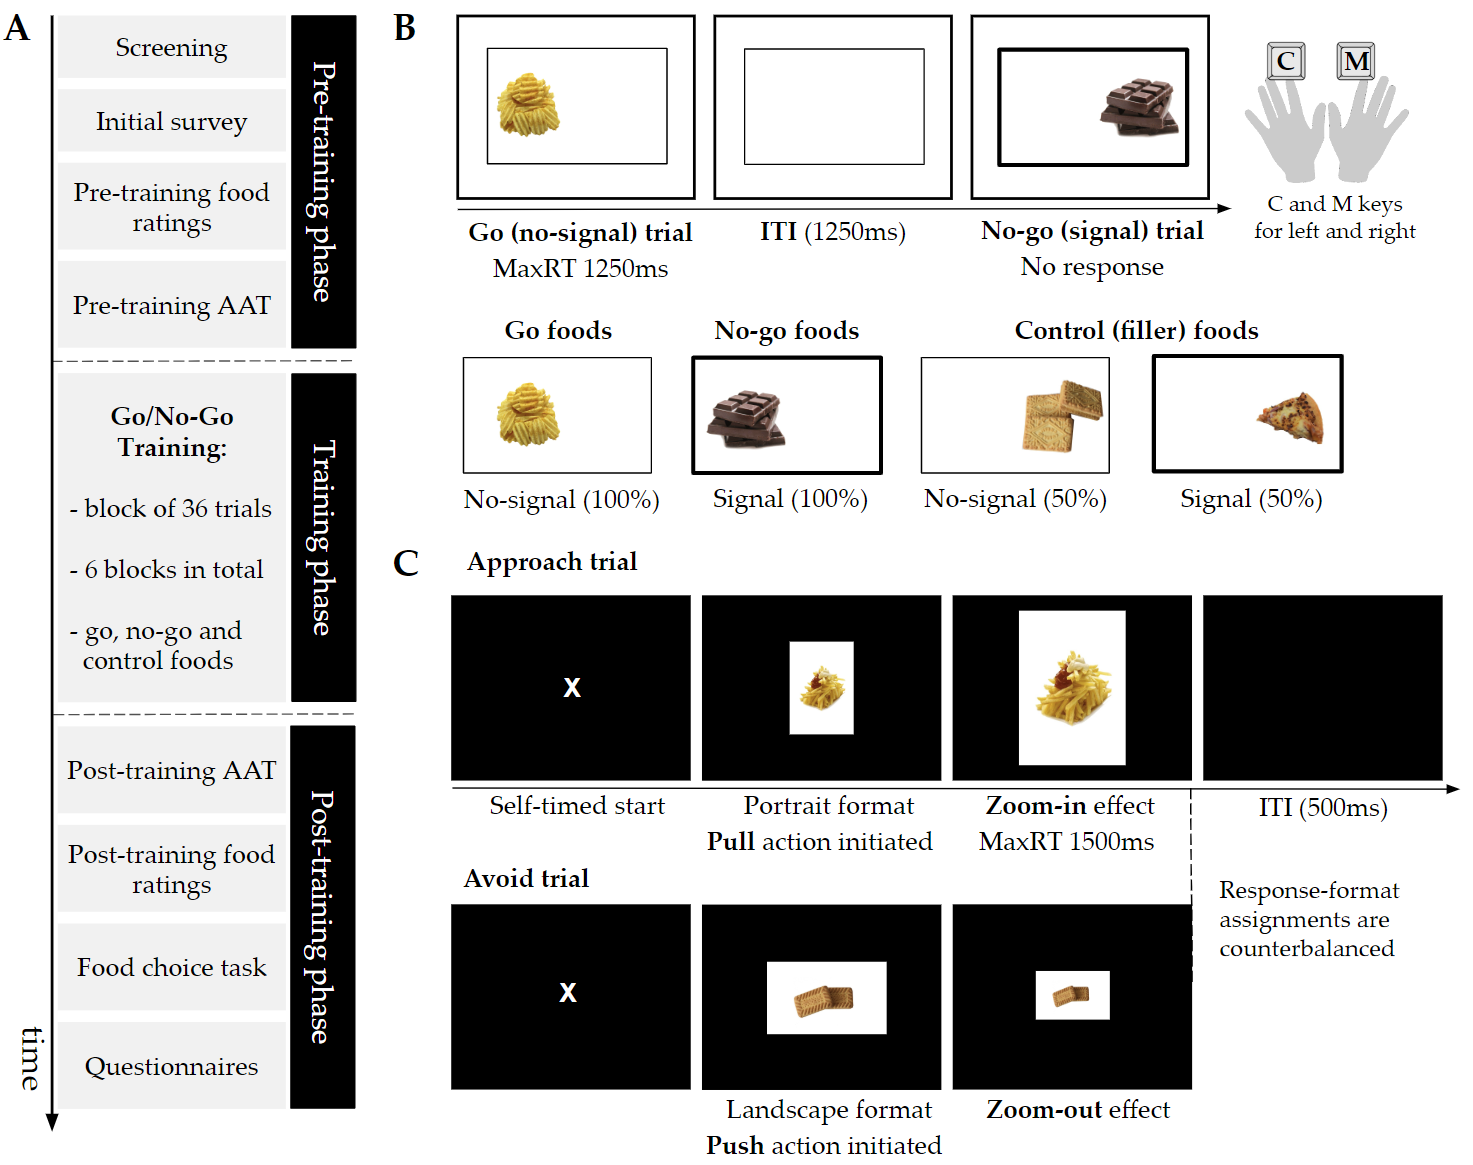
\includegraphics[width=\linewidth]{figures/Figure1.png}
\caption{\textbf{Schematic diagram of the study procedure, go/no-go training and approach-avoidance tasks.} \textbf{A.} After completing the screening and initial survey, participants rated all food stimuli for taste and proceeded to perform the pre-training approach-avoidance task (AAT) blocks. In the training phase, participants completed six blocks of go/no-go training. The post-training AAT blocks were then presented and followed by food liking ratings. At the end of the study, participants completed a short food choice task and several questionnaires, in random order. \textbf{B.} The go/no-go training paradigm involved go (no-signal) and no-go (signal) trials that occured with equal probability. On go trials, participants had to respond within 1250ms by pressing the 'C' and 'M' keys to indicate the picture location (left or right, respectively). On no-go trials, participants were instructed not to respond at all. The inter-trial interval (ITI) was 1250ms. Food categories were randomly assigned to three conditions. Go foods were only paired with no-signal trials and no-go foods were always associated with no-signal trials. Control, or filler, foods were presented in both signal and no-signal trials (50\%, 50\%).}
\label{fig:procedure}
\end{figure}
\clearpage
\begin{figure}
    \ContinuedFloat
    \captionsetup{labelformat=empty}
    \caption{\textbf{C.} In the approach-avoidance task, participants were asked to judge the format of the presented rectangle, which would either be portrait or landscape. Response-format assignements were approximately counterbalanced across participants. As an example, on approach trials a participant would have to pull the mouse towards them when the picture was in portrait format (approach trial) and push it away from them when the picture was in landscape format. Push and pull actions were paired with visual feedback, that is, zoom-out and zoom-in effects respectively. The maximum reaction time (maxRT) was 1500ms and the ITI set to 500ms.}
\end{figure}

\hypertarget{gng}{%
\subsection{Go/No-go training}\label{gng}}

\par

The Go/No-Go (GNG) training paradigm involved \enquote{go} and \enquote{no-go} responses to six pre-selected appetitive food categories. Food categories differed in terms of taste, so that three foods were savoury (i.e., pizza, crisps, chips) and three foods were sweet (i.e., biscuits, chocolate, cake)\footnote{All study materials are openly available at https://osf.io/wcf4r/}. Two food categories were randomly assigned to each training condition (go, no-go, filler foods) in the beginning of the experiment and food taste was counterbalanced so that each condition had one sweet and one savoury food. There were three training conditions according to the mapping of foods to signal (no-go) and no-signal (go) trials in the GNG paradigm. All go foods appeared in go trials and all no-go foods were presented with the signal (see Figure 1, panel C). Control foods appeared on both go and no-go trials with equal probability (i.e., 50\% signal and 50\% no-signal trial mapping). Each food category had three exemplars which appeared twice in each block.

\par

All foods were presented on either the left or right hand side of the screen within a rectangle for 1250ms (see Figure 1, panel B). Participants were asked to respond to the location of the food as quickly and as accurately as possible by pressing the \enquote{C} and \enquote{M} buttons on the keyboard with their left and right index fingers, respectively. The central rectangle remained on the screen throughout the training, including the inter-trial-interval (ITI), which was 1250ms. On signal trials, the rectangle turned \enquote{bold}, indicating that participants should withhold their response. In line with the GNG training paradigm, this signal appeared on stimulus onset (i.e., no delay between stimulus and signal) and stayed on the screen until the end of the trial. A correct response on no-signal trials was registered when participants responded accurately to the location of the food within the time limit and a successful stop (i.e., correct signal trial) was considered when participants did not respond during the trial time window at all. Incorrect responses in no-signal trials refer to either to a wrong location judgment or a missed response.
Left and right responses were counterbalanced across all manipulated variables for each type of trial. Training was split into 6 blocks of 36 trials (i.e., 216 trials in total) and lasted approximately 10 minutes with inter-block breaks (15 seconds). Task practice included 12 trials of go and no-go responses (50\%-50\%) and participants responded to the location of grey squares, instead of food pictures. Feedback was presented during the ITI for practice trials only (i.e, \enquote{CORRECT} or \enquote{INCORRECT} in green and red text, respectively).

\hypertarget{aat}{%
\subsection{Approach avoidance task}\label{aat}}

\par

The approach-avoidance task (AAT) was adapted from an existent paradigm (Rinck \& Becker, 2007; R. W. Wiers et al., 2009a), which involves \enquote{pull} (i.e., towards self) and \enquote{push} (i.e, away from self) movements of a joystick. Each type of motor response is paired with visual feedback so that when the joystick is pulled, the image gets bigger (zoom-in) and when it is pushed, the image gets smaller (zoom-out). This \enquote{zooming} effects acts as an exteroceptive cue of either an approach or avoidance response (Neumann \& Strack, 2000). This feature of the joystick AAT complements the proprioceptive properties of the task, where responses requiring arm flexion and extension correspond to approach and avoidance trials, respectively. This task also disambiguates approach and avoidance responses by using the \enquote{zooming} feature (Wiers et al., 2009a). For example, arm extension could indicate an approach response towards an appetitive food (object-reference) or an avoidance response where the food is pushed away from the body/self (self-reference; Phaf, Mohr, Rotteveel, \& Wicherts, 2014). The visual feedback thus provides the self-reference attribute to the responses (e.g., object comes closer to one's body). We also adopted the evaluation-irrelevant feature of the paradigm, whereby participants respond according to the format of (portrait or landscape; e.g., R. W. Wiers et al., 2010a).

\par

AAT responses involved \enquote{push} and \enquote{pull} movements of the computer mouse. Food stimuli were presented in the centre of the screen and participants were instructed to pull the mouse towards them or push the mouse away from them according to whether the image was in portrait or landscape format (see Figure \ref{fig:procedure}). Response-format assignments were approximately counterbalanced across participants\footnote{In the final sample, 74 participants were instructed to pull the mouse towards them (approach) when the picture was in a portrait format and push the mouse away from them (avoid) when it was in a landscape format. 89 participants had the opposite response-format assignment.}. Instructions highlighted moving the mouse cursor until it reaches the end of the screen (top or bottom edge) for a correct response to be registered and making smooth whole-arm movements. Participants had 1500ms to respond after the stimulus appeared. Each trial started with a central \enquote{X} on the screen and participants had to click on it to begin. The ITI was 500 ms and there was no delay between the \enquote{X} click response and the stimulus onset. In order to account for the natural movement of the mouse, pixel tolerance was added to every mouse movement (\(\pm\) 1.25\% of display height), including movement initiation in the beginning of the trial. A response in the AAT was registered as correct only when participants completed the correct action (e.g., pull or push) within the maxRT window and also initiated a movement towards the correct direction. Even if the final response was correct, participants could have changed their movement after making an initial error (e.g., pull instead of push the mouse in an \enquote{avoid} trial) and therefore the direction of their initial movement was also taken into account. The complete RT for an AAT trial was defined as the time from the stimulus onset to the successful completion of a response.

\par

Each AAT block consisted of 72 trials and go, no-go and control foods appeared with equal probability for both \enquote{pull} (approach) and \enquote{push} (avoid) responses. There were 12 approach and 12 avoid trials for each training condition (e.g., no-go) and within those trials, there were six savoury and six sweet foods presented (i.e., 3 exemplars repeated twice). Three AAT blocks were performed before training (AAT\textsubscript{pre}) and three after training (AAT\textsubscript{post}). There was a number of constraints placed on the quasi-random order of the trials within an AAT block. There were no more than three images of the same food category being presented consecutively and no more than three trials with the same picture format in sequence. AAT practice consisted of 10 trials, whereby grey rectangles appeared in either landscape or portrait format. Feedback was presented for practice trials only. The screen background throughout the AAT was black and the task lasted approximately 15 minutes, including the inter-block 15 second breaks. Participants received a reminder of the instructions after each inter-block 15 sec break.

\hypertarget{food_ratings}{%
\subsection{Food liking ratings}\label{food_ratings}}

\par

Participants provided food liking ratings before and after training using a visual analogue scale (VAS). Participants rated all foods included in the GNG paradigm according to how much they liked the taste, ranging from 0 (\enquote{not at all}) to 100 (\enquote{very much}). Task instructions encouraged participants to imagine they were tasting the food in their mouth and then rate how much they liked the taste. The order of the presented foods was randomised and each block consisted of 18 trials. Participants completed a block before training (Liking\textsubscript{pre}) and a block post training (Liking\textsubscript{post}).

\hypertarget{food_choice}{%
\subsection{Food choice task}\label{food_choice}}

Impulsive food choices were assessed using a food choice task adapted from Veling et al. (2013), which included all food categories from the GNG paradigm (two exemplars per category). The twelve foods were presented in a grid layout on the screen and participants had ten seconds to select three foods that they would like to consume the most at that specific time, by clicking on them with the computer mouse. Participants were asked to click on a \enquote{start} button to begin the trial and when a response was registered the selected food stimulus disappeared from the screen. We assumed that this task element would prevent participants from deliberating on their choices and changing their initial responses, which would mean that \textit{impulsive} food choices were no longer measured. However, it shoudl be noted that although participants were not informed about the hypothetical nature of their choices, it is highly probably that they would not consider their choices consequential (i.e., they would not think that would get a food item after the task).

\hypertarget{survey_questionnaires}{%
\subsection{Survey \& Questionnaires}\label{survey_questionnaires}}

\par

Eligible participants were presented with an initial survey to record demographics and other variables for exploratory analyses. The survey constited of questions height and weight measurements to calculate participant's body-mass-index (BMI; kg/m\textsuperscript{2}), the number of hours since their last meal (\enquote{less than 3 hours ago}, \enquote{3-5 hours ago}, \enquote{5-10 hours ago}, \enquote{more than 10 hours ago}) and hunger state at the the time of the study (VAS:1=\enquote{Not at all} to 9=\enquote{Very}). Gender was also recorded with the options of male, female, transgender male, transgender female, gender variant/non-conforming, and an open ended text response for \enquote{other}.

\par

Several questionnaires were completed by the participants at the end of the study for exploratory analyses, as part of the undergraduate student projects of the GW4 Undergraduate Psychology Consortium 2017/2018. The Barratt Impulsivity Scale (BIS-15; Spinella, 2007) was introduced to explore the relationship between training outcomes and impulsivity. We also examined a distinctive element of general trait self-control, referred to as stop control, using the Stop Control Scale (SCS; De Boer, van Hooft, \& Bakker, 2011). Other administered questionnaires included the Food Cravings Questionnaire - Trait - reduced (FCQ-T-r; Meule, Hermann, \& Kübler, 2014), Perceived Stress Scale (PSS; Cohen, Kamarck, \& Mermelstein, 1983) and the \enquote{food} and \enquote{money} subscales from the Delaying Gratification Inventory (DGI; Hoerger, Quirk, \& Weed, 2011).

\hypertarget{analyses}{%
\section{Analyses}\label{analyses}}

\hypertarget{measures-indices}{%
\subsection{Measures \& indices}\label{measures-indices}}

\par

Reaction time and accuracy data from the GNG blocks were recorded for all design cells for an exploratory assessment of training performance (see \hl{[section]}). The mean error rates in no-signal and signal trials as well as mean reaction time in no-signal trials (GoRT) informed participant exclusions from all analyses (see \textit{\nameref{data_exclusions}}). For the contingency learning manipulation check (H3, H4), we measured the average proportion of successful stops from signal trials for no-go foods and control foods which were paired with a signal (controlnogo) and the mean GoRTs for each participant from go and controlgo trials.

\par

Performance in the AAT\textsubscript{pre} and AAT\textsubscript{post} blocks was considered only for correct responses. We calculated median RTs for \enquote{push} and \enquote{pull} responses on all training condition levels, at a participant level\footnote{RTs were recorded continuously from movement initiation to response completion with samples every 33ms (two display refresh rates) to allow dynamic zoom-in/zoom-out effects based on participants' mouse movements. However, a bug was encountered with the version of the software and the temporal resolution at which coordinates and times were recorded was reduced. For this reason, we used linear interpolation to increase our samples to 100 for every trial and obtain more precise RT measures. All details regarding this procedure and the software bug can be found in our analyses scripts.}. Medians were used instead of means as they are less sensitive to outliers in RT distributions and in line with previous literature (R. W. Wiers et al., 2009b, 2010b). The approach-avoid bias score for each condition was calculated as the difference between the median RTs for \enquote{push} and' pull' responses (MedianRT\textsubscript{push}- MedianRT\textsubscript{pull}). Bias scores were computed for both AAT\textsubscript{pre} and AAT\textsubscript{post} blocks. Positive scores indicate an approach bias towards the foods of interest and negative scores reflect avoidance for those foods. Change scores for approach-avoid biases from pre-to post-training (\(\Delta\)AAT bias score) were calculated for pre-registered analyses (H1). The proportion of correct responses for each AAT design cell informed participant exclusions.

\par

Participants were required to choose three foods out of twelve in the food choice task and selections could vary in their number for each training condition (go, no-go, control). Food choices were therefore normalised according to the total number of responses per participant (i.e., proportion). For the analyses of food choices, we compared the mean proportions of choices (calculated per participant relative to their total number of choices) between each training condition. Food rating VAS scores were averaged (mean) across the two foods per training condition (i.e., sweet and savoury foods for go, no-go and control conditions) and the three exemplars of each food. Changes in food liking were examined in terms of change scores (\(\Delta\)Food liking score) from pre-to-post training.

\hypertarget{data_exclusions}{%
\subsection{Data exclusions}\label{data_exclusions}}

\par

Participant-level data exclusions were conducted based on GNG training and AAT performance. Participants who met any of the following criteria were excluded from all respective analyses. We excluded participants who had a mean GoRT greater than three standard deviations from the group mean and percentage of correct responses in no-signal trials less than 85\%. Participants were also excluded if their percentage of errors in signal trials was greater than three standard deviations from the group mean and percentage of errors in either pre- or post- AAT blocks greater than 0.25. Additionally, participants who submitted a food rating of 50 (i.e., neutral) for 24 or more trials wither pre-or post-training would not be included as we assumed that multiple such responses would indicate that participants used the default setting of the VAS and purposefully skipped the rating trials.

\hypertarget{prereg_analyses}{%
\subsection{Pre-registered analyses}\label{prereg_analyses}}

\par

Data pre-processing and analyses were conducted in RStudio (RStudio Team, 2016) and JASP (JASP Team, 2018). Pre-registered analyses are described under their pre-specified hypotheses, as presented in \textit{\nameref{hypotheses}}. Directional hypotheses will be tested via Bayesian paired-samples t-tests (e.g., see H1a and H1b below).

\noindent H1. The effect of training condition on the change in approach-avoid bias scores from pre-to post-training was examined using a Bayesian Repeated Measures ANOVA with the default prior settings (Rouder, Engelhardt, McCabe, \& Morey, 2016; Rouder, Morey, Speckman, \& Province, 2012) and participants treated as a nuisance term.

\begin{itemize}
\item[H1a.] $\Delta$AAT\textsubscript{nogo} <  $\Delta$AAT\textsubscript{control}  
\item[H1b.] $\Delta$AAT\textsubscript{go} >  $\Delta$AAT\textsubscript{control}
\end{itemize}

\noindent H2. Two Bayesian paired samples t-tests were conducted for the mean proportions of selected foods in the go and no-go training condition compared to the control.

\begin{itemize}
\item[H2a.] p(no-go) < p(control)
\item[H2b.] p(go) > p(control)
\end{itemize}

\noindent H3. The effect of training condition on the change in food liking from pre-to post-training was examined using a Bayesian Repeated Measures ANOVA, consistent with H1.

\begin{itemize}
\item[H3a.] $\Delta$Liking\textsubscript{nogo} < $\Delta$Liking\textsubscript{control}
\item[H3b.] $\Delta$Liking\textsubscript{go} > $\Delta$Liking\textsubscript{control}
\end{itemize}

\noindent H4. Contingency learning during go/no-go training was examined using Bayesian paired-samples t-tests for the percentage of successful inhibition trials and go reaction times.

\begin{itemize}
\item[H4a.] PCsignal\textsubscript{nogo} > PCsignal\textsubscript{control-nogo}
\item[H4b.] GoRT\textsubscript{go} < GoRT\textsubscript{control-go}
\end{itemize}

The evidential value of confirmatory findings was solely determined by the Bayesian tests outlined in this section, as previously explained (see \textit{\nameref{sampling_plan}}. Frequentist tests were conducted for reporting purposes and further the reproducibility of findings (e.g., potential use in meta-analyses). Frequentist paired samples t-tests were two-tailed, in line with the reported power analysis and for pairwise comparisons following the repeated measures ANOVAs for H1 and H3 were corrected for multiple comparisons (Bonferroni).
\hl{make sure we mention that frequentist tests will be two-tailed in line with our power analysis and what we pre-registered of course}

\hypertarget{results}{%
\section{Results}\label{results}}

\hypertarget{sample-characteristics}{%
\subsection{Sample characteristics}\label{sample-characteristics}}

The final sample for pre-registered analyses consisted of 163 participants. Detailed participant-level exclusions are presented in Figure A1.

\hypertarget{confirmatory-findings-for-training-outcomes}{%
\subsection{Confirmatory findings for training outcomes}\label{confirmatory-findings-for-training-outcomes}}

\par

We found \emph{strong} evidence for the absence of a general effect of go/no-go training condition on the change in approach-bias scores {[}\emph{BF}\textsubscript{01} = 15.99; \emph{F}(2, 324) = 1.01, \emph{p} = 0.365{]}. There was moderate evidence (\emph{BF}\textsubscript{01} = 9.31) that the change in bias scores for no-go foods (\(\Delta\)AAT\textsubscript{nogo}; \emph{M} = -3.31, \emph{SD} = 62.91) was not reduced compared to the change for filler foods (\(\Delta\)AAT\textsubscript{control}; \emph{M} = -1.81, \emph{SD} = 59.55), as shown in Table \hl{add label here}. Similar to H1a, we found \emph{strong} evidence (\emph{BF}\textsubscript{01} = 25.73) for the null compared to the alternative for H1b. The change in bias scores for go foods (\(\Delta\)AAT\textsubscript{go}; \emph{M} = -10.47, \emph{SD} = 59.57) was not greater than the change for filler foods.

\par

The effect of training on impulsive food choices was examined for no-go and go foods compared to control, as stated in H2a and H2b respectively. There was \emph{extreme} evidence that the probability of choosing a no-go food (\emph{M} = 0.21, \emph{SD} = 0.27) was reduced compared to the probability of choosing a filler food (\emph{M} = 0.36; \emph{SD} = 0.31) after training {[}H2a; \emph{BF}\textsubscript{10} = 247.78; \emph{t}(161) = -3.93, \emph{p} \textless{} .001, \emph{d} = -0.31, 95\% CI for \emph{d} = -0.47, -0.15\footnote{Shapiro-Wilk tests suggested deviation from normality (\textit{p} < .001) and the results from the Wilcoxon signed-ranked tests are reported here. H2a: \textit{W} = 1875.00, \textit{p} < .001, \textit{r} = -0.716; H2b: \textit{W} = 4663.00, \textit{p} = 0.048, \textit{r} = -0.294}{]}. In contrast, we only obtained \emph{anecdotal} evidence that probability of choosing a go food (\emph{M} = 0.44; \emph{SD} = 0.33) was not greater than the probability of choosing a filler food after training {[}\emph{BF}\textsubscript{01} = 1.18, \emph{t}(161) = 1.82, \emph{p} = 0.070, \emph{d} = 0.14, 95\% CI for \emph{d} = -0.01, 0.30{]}.

\hypertarget{manipulation-checks-for-training}{%
\subsection{Manipulation checks for training}\label{manipulation-checks-for-training}}

\par
\hl{we pre-registered an anova too for this}

In order to validate whether the implemented go/no-go training paradigm led to stimulus-response associations (i.e., contingency learning) we first tested whether the percentage of correct responses for no-go foods (i.e., successful inhibitions) would be greater compared to the percentage of correct responses for filler foods associated with signal trials (H4a). There was \emph{extreme} evidence that participants had on average more successful inhibitions for no-go foods (PCsignal\textsubscript{nogo}; \emph{M} = 0.97, \emph{SD} = 0.03) than filler foods
(PCsignal\textsubscript{control-nogo}; \emph{M} = 0.96, \emph{SD} = 0.04) {[}\emph{BF}\textsubscript{10} = 140.30, \hl{..put in a table?}{]} For H4b, we tested whether mean reaction times would be reduced for go foods (GoRT\textsubscript{go}; \emph{M} = 507.00, \emph{SD} = 70.48) compared to filler foods associated with no-signal trials (GoRT\textsubscript{control-go}; \emph{M} = 515.00, \emph{SD} = 75.51) and there was \emph{extreme} evidence for such an effect. Therefore, contingency learning was observed in the employed GNG paradigm for both reaction time and accuracy outcomes.

\par

As a second manipulation check for training outcomes, we investigated whether GNG changed the evaluations of foods associated with signal and no-signal trials compared to the evaluations of filler foods which were paired with either type of trial with equal probability (control). \hl{maybe point for discussion: if evaluations are already high we might expect to see a ceiling effect- as reported in chen's latest papers- what we didn't test for and might be worth looking at is no-go versus go! extra validation- can strengthn the claim that stimulus devaluation occured}

The change in liking scores from pre-to post-training for nogo foods (\(\Delta\)Liking\textsubscript{nogo}; \emph{M} = -4.16; \emph{SD} = 9.51) was only slightly reduced compared to change in liking for filler foods (\(\Delta\)Liking\textsubscript{control}; \emph{M} = -2.61, \emph{SD} = 8.77), and there was only anecdotal evidence for this effect {[}H3a; \emph{BF}\textsubscript{10} = 2.65, \emph{t}(162) = -2.38, \emph{p} = 0.019, \emph{d} = -0.19, 95\% CI for \emph{d} = -0.34, -0.03\footnote{Although data transformations or alternative tests were not pre-registered for the potential violation of the normality assumption, the Shapiro-Wilk test showed a deviation from normality (\textit{p} < .001) and thus we also report the results from the Wilcoxon signed-rank tests. The effect size is given by the matched rank biserial correlation (\textit{r}) H3a: \textit{W} = 5907.50, \textit{p} = 0.246, \textit{r} = -0.116; H3b: \textit{W} = 6666.50, \textit{p} = 0.914}, \textit{r} = -0.002{]}. The change in liking scores from pre-to post-training for go foods (\(\Delta\)Liking\textsubscript{go}; \emph{M} = -2.87, \emph{SD} = 10.15), however, was not greater than the change for filler foods as originally expected. \hl{this is not surprising as there may be a ceiling effect in how much these foods can be liked more.. see chen for discussion} Instead, there was \emph{strong} evidence for the null hypothesis compared to the alternative {[}H3b; \emph{BF}\textsubscript{01} = 14.95, \emph{t}(162) = -0.37, \emph{p} = 0.715, \emph{d} = -0.03, 95\% CI for \emph{d} = -0.18, 0.13{]}.

\hypertarget{discussion}{%
\section{Discussion}\label{discussion}}

\newpage

\include{Appendix}

\hypertarget{references}{%
\section{References}\label{references}}

\begingroup
\setlength{\parindent}{-0.5in}
\setlength{\leftskip}{0.5in}

\hypertarget{refs}{}
\leavevmode\hypertarget{ref-adams_training_2017}{}%
Adams, R. C., Lawrence, N. S., Verbruggen, F., \& Chambers, C. D. (2017). Training response inhibition to reduce food consumption: Mechanisms, stimulus specificity and appropriate training protocols. \emph{Appetite}, \emph{109}, 11--23. \url{https://doi.org/10.1016/j.appet.2016.11.014}

\leavevmode\hypertarget{ref-allom_does_2016}{}%
Allom, V., Mullan, B., \& Hagger, M. (2016). Does inhibitory control training improve health behaviour? A meta-analysis. \emph{Health Psychol. Rev.}, \emph{10}(2), 168--186. \url{https://doi.org/10.1080/17437199.2015.1051078}

\leavevmode\hypertarget{ref-becker_approach_2015-1}{}%
Becker, D., Jostmann, N. B., Wiers, R. W., \& Holland, R. W. (2015). Approach avoidance training in the eating domain: Testing the effectiveness across three single session studies. \emph{Appetite}, \emph{85}(June 2015), 58--65. \url{https://doi.org/10.1016/j.appet.2014.11.017}

\leavevmode\hypertarget{ref-benjamin_redefine_2017}{}%
Benjamin, D. J., Berger, J. O., Johannesson, M., Nosek, B. A., Wagenmakers, E.-J., Berk, R., \ldots{} Johnson, V. E. (2018). Redefine statistical significance. \emph{Nature Human Behaviour}, \emph{2}, 6--10. \url{https://doi.org/10.1038/s41562-017-0189-z}

\leavevmode\hypertarget{ref-button_power_2013}{}%
Button, K. S., Ioannidis, J. P. A., Mokrysz, C., Nosek, B. A., Flint, J., Robinson, E. S. J., \& Munaf\a`o, M. R. (2013). Power failure: Why small sample size undermines the reliability of neuroscience. \emph{Nat. Rev. Neurosci.}, \emph{14}(5), 365--376. \url{https://doi.org/10.1038/nrn3475}

\leavevmode\hypertarget{ref-chen_when_2018}{}%
Chen, Z., Holland, R., Quandt, J., Dijksterhuis, A., \& Veling, H. (2018a). When mere action versus inaction leads to robust preference change. \url{https://doi.org/10.17605/OSF.IO/ZY9W3}

\leavevmode\hypertarget{ref-chenWhenMereAction2018}{}%
Chen, Z., Holland, R., Quandt, J., Dijksterhuis, A., \& Veling, H. (2018b). When mere action versus inaction leads to robust preference change. \url{https://doi.org/10.17605/OSF.IO/ZY9W3}

\leavevmode\hypertarget{ref-chen_how_2016-1}{}%
Chen, Z., Veling, H., Dijksterhuis, A., \& Holland, R. W. (2016a). How does not responding to appetitive stimuli cause devaluation: Evaluative conditioning or response inhibition? \emph{Journal of Experimental Psychology: General}, \emph{145}(12), 1687--1701. \url{https://doi.org/10.1037/xge0000236}

\leavevmode\hypertarget{ref-chen_how_2016}{}%
Chen, Z., Veling, H., Dijksterhuis, A., \& Holland, R. W. (2016b). How does not responding to appetitive stimuli cause devaluation: Evaluative conditioning or response inhibition? \emph{Journal of Experimental Psychology: General}, \emph{145}(12), 1687--1701. \url{https://doi.org/10.1037/xge0000236}

\leavevmode\hypertarget{ref-cohenGlobalMeasurePerceived1983}{}%
Cohen, S., Kamarck, T., \& Mermelstein, R. (1983). A global measure of perceived stress. \emph{Journal of Health and Social Behavior}, \emph{24}(4), 385--396.

\leavevmode\hypertarget{ref-deboerStopStartControl2011}{}%
De Boer, B. J., van Hooft, E. A. J., \& Bakker, A. B. (2011). Stop and start control: A distinction within self-control. \emph{European Journal of Personality}, \emph{25}(5), 349--362. \url{https://doi.org/10.1002/per.796}

\leavevmode\hypertarget{ref-faul_statistical_2009}{}%
Faul, F., Erdfelder, E., Buchner, A., \& Lang, A.-G. (2009). Statistical power analyses using G*Power 3.1: Tests for correlation and regression analyses. \emph{Behav. Res. Methods}, \emph{41}(4), 1149--1160. \url{https://doi.org/10.3758/BRM.41.4.1149}

\leavevmode\hypertarget{ref-hoergerDevelopmentValidationDelaying2011}{}%
Hoerger, M., Quirk, S. W., \& Weed, N. C. (2011). Development and validation of the Delaying Gratification Inventory. \emph{Psychological Assessment}, \emph{23}(3), 725--738. \url{https://doi.org/10.1037/a0023286}

\leavevmode\hypertarget{ref-houben_training_2011}{}%
Houben, K., \& Jansen, A. (2011). Training inhibitory control. A recipe for resisting sweet temptations. \emph{Appetite}, \emph{56}(2), 345--349. \url{https://doi.org/10.1016/j.appet.2010.12.017}

\leavevmode\hypertarget{ref-houben_chocolate_2015}{}%
Houben, K., \& Jansen, A. (2015). Chocolate equals stop: Chocolate-specific inhibition training reduces chocolate intake and go associations with chocolate. \emph{Appetite}, \emph{87}, 318--323. \url{https://doi.org/10.1016/j.appet.2015.01.005}

\leavevmode\hypertarget{ref-houben_too_2012}{}%
Houben, K., Nederkoorn, C., \& Jansen, A. (2012). Too tempting to resist? Past success at weight control rather than dietary restraint determines exposure-induced disinhibited eating. \emph{Appetite}, \emph{59}(2), 550--555. \url{https://doi.org/10.1016/j.appet.2012.07.004}

\leavevmode\hypertarget{ref-houben_eating_2014}{}%
Houben, K., Nederkoorn, C., \& Jansen, A. (2014). Eating on impulse: The relation between overweight and food-specific inhibitory control. \emph{Obesity}, \emph{22}(5), 2013--2015. \url{https://doi.org/10.1002/oby.20670}

\leavevmode\hypertarget{ref-JASP2018:1}{}%
JASP Team. (2018). JASP (Version 0.10.0){[}Computer software{]}.

\leavevmode\hypertarget{ref-jones_inhibitory_2016}{}%
Jones, A., Di Lemma, L. C. G., Robinson, E., Christiansen, P., Nolan, S., Tudur-Smith, C., \& Field, M. (2016a). Inhibitory control training for appetitive behaviour change: A meta-analytic investigation of mechanisms of action and moderators of effectiveness. \emph{Appetite}, \emph{97}, 16--28. \url{https://doi.org/10.1016/j.appet.2015.11.013}

\leavevmode\hypertarget{ref-jonesInhibitoryControlTraining2016}{}%
Jones, A., Di Lemma, L. C. G., Robinson, E., Christiansen, P., Nolan, S., Tudur-Smith, C., \& Field, M. (2016b). Inhibitory control training for appetitive behaviour change: A meta-analytic investigation of mechanisms of action and moderators of effectiveness. \emph{Appetite}, \emph{97}, 16--28. \url{https://doi.org/10.1016/j.appet.2015.11.013}

\leavevmode\hypertarget{ref-kakoschke_combined_2015-1}{}%
Kakoschke, N., Kemps, E., \& Tiggemann, M. (2015). Combined effects of cognitive bias for food cues and poor inhibitory control on unhealthy food intake. \emph{Appetite}, \emph{87}, 358--364. \url{https://doi.org/10.1016/j.appet.2015.01.004}

\leavevmode\hypertarget{ref-lavagnino_inhibitory_2016}{}%
Lavagnino, L., Arnone, D., Cao, B., Soares, J. C., \& Selvaraj, S. (2016). Inhibitory control in obesity and binge eating disorder: A systematic review and meta-analysis of neurocognitive and neuroimaging studies. \emph{Neurosci. Biobehav. Rev.}, \emph{68}, 714--726. \url{https://doi.org/10.1016/j.neubiorev.2016.06.041}

\leavevmode\hypertarget{ref-lawrence_nucleus_2012-1}{}%
Lawrence, N. S., Hinton, E. C., Parkinson, J. A., \& Lawrence, A. D. (2012). Nucleus accumbens response to food cues predicts subsequent snack consumption in women and increased body mass index in those with reduced self-control. \emph{NeuroImage}, \emph{63}(1), 415--422. \url{https://doi.org/10.1016/j.neuroimage.2012.06.070}

\leavevmode\hypertarget{ref-lawrence_training_2015}{}%
Lawrence, N. S., O'Sullivan, J., Parslow, D., Javaid, M., Adams, R. C., Chambers, C. D., \ldots{} Verbruggen, F. (2015a). Training response inhibition to food is associated with weight loss and reduced energy intake. \emph{Appetite}, \emph{95}, 17--28. \url{https://doi.org/10.1016/j.appet.2015.06.009}

\leavevmode\hypertarget{ref-lawrenceTrainingResponseInhibition2015}{}%
Lawrence, N. S., O'Sullivan, J., Parslow, D., Javaid, M., Adams, R. C., Chambers, C. D., \ldots{} Verbruggen, F. (2015b). Training response inhibition to food is associated with weight loss and reduced energy intake. \emph{Appetite}, \emph{95}, 17--28. \url{https://doi.org/10.1016/j.appet.2015.06.009}

\leavevmode\hypertarget{ref-lawrence_stopping_2015-3}{}%
Lawrence, N. S., Verbruggen, F., Morrison, S., Adams, R. C., \& Chambers, C. D. (2015a). Stopping to food can reduce intake. Effects of stimulus-specificity and individual differences in dietary restraint. \emph{Appetite}, \emph{85}, 91--103. \url{https://doi.org/10.1016/j.appet.2014.11.006}

\leavevmode\hypertarget{ref-lawrence_stopping_2015}{}%
Lawrence, N. S., Verbruggen, F., Morrison, S., Adams, R. C., \& Chambers, C. D. (2015b). Stopping to food can reduce intake. Effects of stimulus-specificity and individual differences in dietary restraint. \emph{Appetite}, \emph{85}, 91--103. \url{https://doi.org/10.1016/j.appet.2014.11.006}

\leavevmode\hypertarget{ref-lee_bayesian_2013}{}%
Lee, M. D., \& Wagenmakers, E.-J. (2013). \emph{Bayesian Cognitive Modeling: A Practical Course}. Cambridge University Press. \url{https://doi.org/10.1017/CBO9781139087759}

\leavevmode\hypertarget{ref-meule_short_2014}{}%
Meule, A., Hermann, T., \& Kübler, A. (2014). A short version of the Food Cravings QuestionnaireTrait: The FCQ-T-reduced. \emph{Frontiers in Psychology}, \emph{5}. \url{https://doi.org/10.3389/fpsyg.2014.00190}

\leavevmode\hypertarget{ref-richard_d._morey_verbal_2015}{}%
Morey, R. D. (2015). On verbal categories for the interpretation of Bayes factors.

\leavevmode\hypertarget{ref-nederkoorn_specificity_2012}{}%
Nederkoorn, C., Coelho, J. S., Guerrieri, R., Houben, K., \& Jansen, A. (2012). Specificity of the failure to inhibit responses in overweight children. \emph{Appetite}, \emph{59}(2), 409--413. \url{https://doi.org/10.1016/j.appet.2012.05.028}

\leavevmode\hypertarget{ref-neumann_approach_2000}{}%
Neumann, R., \& Strack, F. (2000). Approach and Avoidance: The Influence of Proprioceptive and Exteroceptive Cues on Encoding of Affective Information. \emph{J. Personal. Soc. Psychol.}, \emph{79}(1), 39--48. \url{https://doi.org/10.1037//0022-3514.79.1.39}

\leavevmode\hypertarget{ref-phaf_approach_2014}{}%
Phaf, R. H., Mohr, S. E., Rotteveel, M., \& Wicherts, J. M. (2014). Approach, avoidance, and affect: A meta-analysis of approach-avoidance tendencies in manual reaction time tasks. \emph{Front. Psychol.}, \emph{5}(378), 1--16. \url{https://doi.org/10.3389/fpsyg.2014.00378}

\leavevmode\hypertarget{ref-rinck_approach_2007}{}%
Rinck, M., \& Becker, E. S. (2007). Approach and avoidance in fear of spiders. \emph{Journal of Behavior Therapy and Experimental Psychiatry}, \emph{38}(2), 105--120. \url{https://doi.org/10.1016/j.jbtep.2006.10.001}

\leavevmode\hypertarget{ref-rouderModelComparisonANOVA2016}{}%
Rouder, J. N., Engelhardt, C. R., McCabe, S., \& Morey, R. D. (2016). Model comparison in ANOVA. \emph{Psychon. Bull. Rev.}, \emph{23}(6), 1779--1786. \url{https://doi.org/10.3758/s13423-016-1026-5}

\leavevmode\hypertarget{ref-rouderDefaultBayesFactors2012}{}%
Rouder, J. N., Morey, R. D., Speckman, P. L., \& Province, J. M. (2012). Default Bayes factors for ANOVA designs. \emph{Journal of Mathematical Psychology}, \emph{56}(5), 356--374. \url{https://doi.org/10.1016/j.jmp.2012.08.001}

\leavevmode\hypertarget{ref-rstudio}{}%
RStudio Team. (2016). \emph{RStudio: Integrated Development Environment for R}. Boston, MA: RStudio, Inc.

\leavevmode\hypertarget{ref-schumacher_bias_2016}{}%
Schumacher, S. E., Kemps, E., \& Tiggemann, M. (2016). Bias modification training can alter approach bias and chocolate consumption. \emph{Appetite}, \emph{96}, 219--224. \url{https://doi.org/10.1016/j.appet.2015.09.014}

\leavevmode\hypertarget{ref-spinellaNormativeDataShort2007}{}%
Spinella, M. (2007). Normative Data and a Short Form of the Barratt Impulsiveness Scale. \emph{International Journal of Neuroscience}, \emph{117}(3), 359--368. \url{https://doi.org/10.1080/00207450600588881}

\leavevmode\hypertarget{ref-strack_reflective_2004}{}%
Strack, F., \& Deutsch, R. (2004). Reflective and Impulsive Determinants of Social Behavior. \emph{Personality and Social Psychology Review}, \emph{8}(3), 28.

\leavevmode\hypertarget{ref-veling_using_2011}{}%
Veling, H., Aarts, H., \& Papies, E. K. (2011). Using stop signals to inhibit chronic dieters' responses toward palatable foods. \emph{Behav. Res. Ther.}, \emph{49}(11), 771--780. \url{https://doi.org/10.1016/j.brat.2011.08.005}

\leavevmode\hypertarget{ref-veling_stop_2013}{}%
Veling, H., Aarts, H., \& Stroebe, W. (2013). Stop signals decrease choices for palatable foods through decreased food evaluation. \emph{Front. Psychol.}, \emph{4}(875), 1--7. \url{https://doi.org/10.3389/fpsyg.2013.00875}

\leavevmode\hypertarget{ref-veling_training_2017-1}{}%
Veling, H., Chen, Z., Tombrock, M. C., M. Verpaalen, I. a., Schmitz, L. I., Dijksterhuis, A., \& Holland, R. W. (2017). Training Impulsive Choices for Healthy and Sustainable Food. \emph{J. Exp. Psychol. Appl.}, \emph{23}(1), 1--14. \url{https://doi.org/10.1037/xap0000112}

\leavevmode\hypertarget{ref-veling_when_2008}{}%
Veling, H., Holland, R. W., \& van Knippenberg, A. (2008). When approach motivation and behavioral inhibition collide: Behavior regulation through stimulus devaluation. \emph{Journal of Experimental Social Psychology}, \emph{44}(4), 1013--1019. \url{https://doi.org/10.1016/j.jesp.2008.03.004}

\leavevmode\hypertarget{ref-veling_what_2017}{}%
Veling, H., Lawrence, N. S., Chen, Z., van Koningsbruggen, G. M., \& Holland, R. W. (2017). What Is Trained During Food Go/No-Go Training? A Review Focusing on Mechanisms and a Research Agenda. \emph{Curr. Addict. Reports}, \emph{4}(1), 35--41. \url{https://doi.org/10.1007/s40429-017-0131-5}

\leavevmode\hypertarget{ref-veling_targeting_2014}{}%
Veling, H., van Koningsbruggen, G. M., Aarts, H., \& Stroebe, W. (2014). Targeting impulsive processes of eating behavior via the internet. Effects on body weight. \emph{Appetite}, \emph{78}, 102--109. \url{https://doi.org/10.1016/j.appet.2014.03.014}

\leavevmode\hypertarget{ref-wiers_relatively_2009}{}%
Wiers, R. W., Rinck, M., Dictus, M., \& Van Den Wildenberg, E. (2009a). Relatively strong automatic appetitive action-tendencies in male carriers of the OPRM1 G-allele. \emph{Genes, Brain Behav.}, \emph{8}(1), 101--106. \url{https://doi.org/10.1111/j.1601-183X.2008.00454.x}

\leavevmode\hypertarget{ref-wiersRelativelyStrongAutomatic2009}{}%
Wiers, R. W., Rinck, M., Dictus, M., \& Van Den Wildenberg, E. (2009b). Relatively strong automatic appetitive action-tendencies in male carriers of the OPRM1 G-allele. \emph{Genes, Brain Behav.}, \emph{8}(1), 101--106. \url{https://doi.org/10.1111/j.1601-183X.2008.00454.x}

\leavevmode\hypertarget{ref-wiers_retraining_2010}{}%
Wiers, R. W., Rinck, M., Kordts, R., Houben, K., \& Strack, F. (2010a). Retraining automatic action-tendencies to approach alcohol in hazardous drinkers. \emph{Addiction}, \emph{105}(2), 279--287. \url{https://doi.org/10.1111/j.1360-0443.2009.02775.x}

\leavevmode\hypertarget{ref-wiersRetrainingAutomaticAction2010}{}%
Wiers, R. W., Rinck, M., Kordts, R., Houben, K., \& Strack, F. (2010b). Retraining automatic action-tendencies to approach alcohol in hazardous drinkers. \emph{Addiction}, \emph{105}(2), 279--287. \url{https://doi.org/10.1111/j.1360-0443.2009.02775.x}

\endgroup --\textgreater{}


\end{document}
